\documentclass[12pt,a4paper]{article}
\usepackage[utf8]{inputenc}
\usepackage[english]{babel}
\usepackage{amsmath}
\usepackage{amsfonts}
\usepackage{amssymb}
\usepackage{makeidx}
\usepackage{graphicx}
\usepackage{listings}
\usepackage{color}
\usepackage{epstopdf}

\definecolor{dkgreen}{rgb}{0,0.6,0}
\definecolor{gray}{rgb}{0.5,0.5,0.5}
\definecolor{mauve}{rgb}{0.58,0,0.82}
\definecolor{orange}{rgb}{1.0,0.44,0}

\lstdefinelanguage{SPAD}
{keywords={if,then,else,for,in,repeat},
keywords=[2]{Fraction,Integer,Polynomial,RealClosure,Cell, Float, 
             DoubleFloat, CylindricalAlgebraicDecompositionPackage, 
             List},
keywords=[3]{cylindricalDecomposition},
keywordstyle=[2]\color{red},
keywordstyle=[3]\color{orange},
sensitive=true,%
alsoletter={\$},%
comment=[l]{--},%
string=[b]",%
string=[b]'%
}

\lstset{frame=tb,
  language=SPAD,
  aboveskip=3mm,
  belowskip=3mm,
  showstringspaces=false,
  columns=flexible,
  basicstyle={\small\ttfamily},
  numbers=none,
  numberstyle=\tiny\color{gray},
  keywordstyle=\color{blue},
  commentstyle=\color{dkgreen},
  stringstyle=\color{mauve},
  breaklines=true,
  breakatwhitespace=true,
  tabsize=3
}
\author{Kurt Pagani}
\title{Quantifier Elimination in {\tt FriCAS}}
%

\newcommand{\CAD}{{\tt CAD}}
\newcommand{\QE}{{\tt QE}}
\newcommand{\RR}[1]{\mathbb{R}^{#1}}
\newcommand{\QQ}[1]{\mathbb{Q}^{#1}}
\newcommand{\ZZ}[1]{\mathbb{Z}^{#1}}
\newcommand{\KK}[1]{\mathbb{K}^{#1}}


\begin{document}
\maketitle

\begin{abstract}
lorem ipsum. 
\end{abstract}

\section{Introduction}
Let us recall some basic facts and definitions about cylindrical algebraic decomposition (\CAD) and quantifier elimination (\QE).

Let \CAD($\RR n$) denote the set of all cylindrical algebraic 
decompositions of $\RR n$. Then each element represents a partition of
$\RR n$ into finitely many nonempty connected semi-algebraic sets whose 
projections to $\RR m$ are either disjoint or equal. If for instance
$X\in$ \CAD($\RR n$),
\begin{equation}
       \RR n = X_1 \cup \ldots \cup X_l        
\end{equation}
then, letting $\pi_m:\RR n \rightarrow \RR m$, denote the canonical projection, we get an {\sl induced} decomposition $\pi_m(X)\in$ \CAD($\RR m$) and
\begin{equation}
       \RR m = \pi_m(X_1) \cup \ldots \cup \pi_m(X_l).        
\end{equation} 
The abstract definition given above is (usually) equivalent to the original 
concept discovered by George E. Collins \cite{COL73}, however, of little use
to understand the various algorithms. Therefore, we will refer to the 
{\sl standard} work \cite{ACM82} by Arnum, Collins and McCallum for terminology as well as for any results in connection with {\tt CAD}. Moreover, it seems that
Renaud Rioboo's elegant {\tt AXIOM} package is a straightforward implementation
of the algorithm described therein, i.e using McCallum projection. Meanwhile there are some improvements, yet {\tt CAD} still is a tough business, and for certain
problems the original algorithms perform as well. For recent results consult
the two PhD theses \cite{GP11} and \cite{WDJ14} and the literature cited therein.     
And last, a very coherent introduction (as I found) to {\CAD} is given by
Mats Jirstrand in \cite{JM95}.

About 1930, Alfred Tarski discovered \cite{TAR51} that the semi-algebraic 
theory\footnote{{\tt semi} means allowing $\leq,\geq,\neq$ besides $=$.} 
of $\RR n$ admitted quantifier elimination, that is for instance
%
\begin{equation}
       \exists x_{k+1}\forall x_{k+2}\ldots \Phi(x_1,\ldots,x_n) \equiv
       \Psi(x_1,\ldots,x_k),
\end{equation}
%
meaning that a quantified first order formula with or without free variables
can be reduced to an equivalent quantifier free formula. It is widely known
that Tarksi's proof is more of a theoretical value than of being computationally
feasible. As already remarked, it was George Collins who discovered an algorithm
for quantifier elimination based on cylindrical algebraic decomposition. Still,
the complexity depends double-exponentially on the number of variables. For
nomenclature and results with respect to quantifier elimination by {\tt CAD}
we refer to \cite{BCW99} and \cite{ARAG} (esp. chapter 11.3).

\section{Rioboo's CAD Package}
Since September 2014, Renaud Rioboos {\tt CAD} package is also included in 
{\tt FriCAS}, so we have the main ingredient for {\QE} already at hand. In
this section let us try to understand the various functions and to analyze
if and how we can utilize the package to construct a {\tt QE} package. 
Furthermore, we have to mention that there is another package {\tt RealClosure} 
(by the same author \cite{RIO91}) which plays an integral part for {\tt CAD},
but is not in our focus here. 

\subsection{Setup}
In order to use the package we need some preparations:
%
\begin{lstlisting}
 -- Setup CAD
 )clear all

 Q ==> Fraction Integer
 F ==> RealClosure Q
 P ==> Polynomial F
 CADP ==> CylindricalAlgebraicDecompositionPackage(F)
 CELL ==> Cell F

 macro cad == cylindricalDecomposition

\end{lstlisting}
%
Now, our field $F$ is the real closure of $\mathbb Q$, thus has type 
{\tt RealClosure} what is expected by the constructor. The main function 
{\em cylindricalDecomposition} will simply be abbreviated by {\tt cad}, just
for convenience.
%
\begin{lstlisting}
 -- The most simple case p(x)=x
 cad([x],[x])$CADP

 [({x= - 1,true}),({x= 0,false}),({x= 1,true})]
 
 Type: List(Cell(RealClosure(Fraction(Integer))))
\end{lstlisting}
% 
The example above shows all the characteristics of the {\tt cad} function. The
first argument has to be a list of polynomials and the (optional) second argument
can be an ordered list of variables (order sometimes is important regarding
performance), thus it certainly is redundant in the one-dimensional case. 

Now the output is a list of {\em cells} representing a {\tt CAD} of $\RR 1$.
In $\RR n$ the (output) structure of each cell is a follows:
%
\begin{equation}
    (\, \{x_n = v_n, b_n\}, \ldots,  \{x_1 = v_1, b_1\} \,) 
\end{equation}
%
where $(x_1,\ldots,x_n)$ are the coordinates and $(v_1,\ldots,v_n)$ are
the values of a {\em sample point} of the cell. The Boolean values
$(b_1,\ldots,b_n)$ ({\tt true} or {\tt false} in {\tt FriCAS}) indicate
whether the specific coordinate of the sample point is contained in an 
open interval ({\tt true}) or if it is an isolated point ({\tt false})
in the projection of the cell to the corresponding coordinate axis. Notice
that the ordering of the variables is by default $(x_n,\ldots,x_1)$, so
that repeated projection will end up in $x_1$. As remarked, one can change
the order by explicitly provide a second argument to {\tt cad}.   


Since in the example above $n=1$ we (trivially) get the partition
%
\begin{equation}
       \mathbb{R} = (-\infty,0) \cup \{0\} \cup (0,\infty).
\end{equation}
Indeed, the first as well as the third cell has {\em dimension} while
the second one has none. The sample points $\{-1\},\{0\}$ and $\{+1\}$
actually represent the signs of the polynomial $p(x)=x)$ in the cells.
By evaluation we get $(-1,0,1)$. If we use $p(x)=x^2$ instead, the
{\tt CAD} will be the same, however, evaluation at the sample points
will result in $(1,0,1)$. In any case the polynomial will be sign
invariant in each cell.

\subsection{A less trivial example}\label{ex1}
We will follow the introductory example in \cite{JM95}: Given the system
\begin{eqnarray*}
     x^2 + y^2 -1 < 0 \\
     x^3 - y^2 = 0
\end{eqnarray*}
find the set of solutions. It is easy to find the solution (red) but let us
do it by the {\CAD} machinery. Note, however, that the {\CAD}-algorithm in
{\tt FriCAS} uses a more sophisticated projection method than the one 
described in \cite{JM95}, resulting in a projection set of only $3$ 
polynomials instead of $18$.
%
\begin{figure}[!htb]
\centering
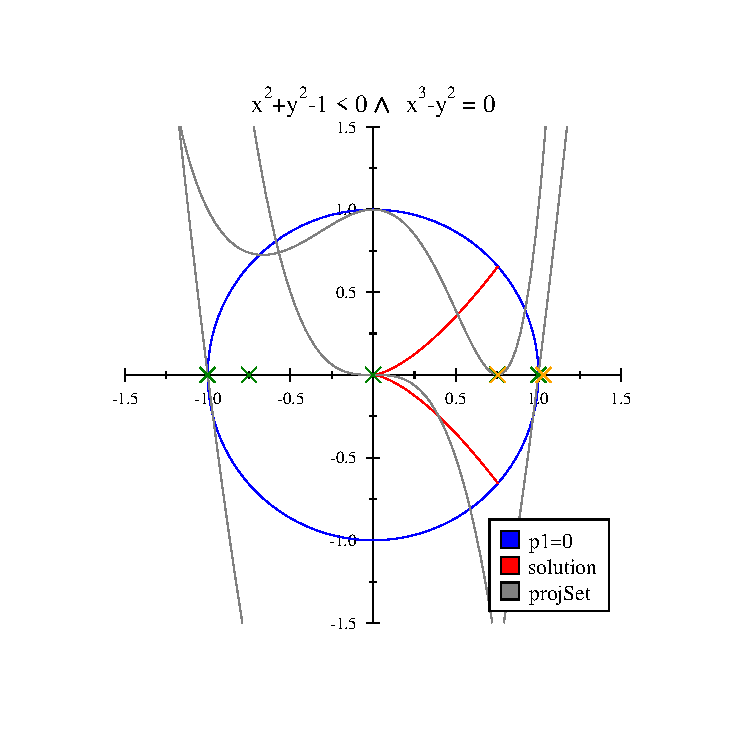
\includegraphics[scale=1.0]{cad1.eps}
\caption{Example 1.}
\label{fig:cad1}
\end{figure}
% 
\begin{lstlisting}
 -- setup as above
 
 p1:=( x^2 + y^2 -1 )$P
 p2:=( x^3 - y^2)$P

 L:=[p1,p2]                 -- list of polynomials
 V:=[x,y]                   -- list of variables (ordered)

 lc:=cad(L,V)$CADP          -- CAD

\end{lstlisting}
%
The output is a {\CAD} with $51$ cells:
%
\begin{verbatim}
  [({y= 0,true},{x= - 3,true}),           -- cell 1 
   ({y= %A2 - 1,true},{x= %A2,false}),    -- cell 2
  ...                                         
\end{verbatim}
%
We immediately see, for example, that the first cell is proper while the
second one must be a vertical line through the {\em algebraic number}
$x=${\tt \%A2}.

\subsection{Some helper functions}
The package provides some more functions of which we will take use to
define some helper functions. 

\subsubsection{List sample points and cell dimensions}
Using the cell functions {\tt samplePoint} and {\tt dimension} we can 
extract a list of sample points and compute a list of cell dimensions by
defining the following functions: 
%
\begin{lstlisting}
 -- list sample points of CAD l
 samplePoints(l) == [samplePoint(l.j) for j in 1..#l]

 -- list dimensions of cells in CAD l
 dimensions(l) == [dimension(l.j) for j in 1..#l]
\end{lstlisting}
%
Applying the two functions to the {\CAD} of our example yields:
%
\begin{verbatim}
 samplePoints lc
   [[0,- 3], [%A2 - 1,%A2], [0,%A2], [- %A2 + 1,%A2], ...] 
   Type: List(List(RealClosure(Fraction(Integer)))) 
\end{verbatim}
and the dimension of each cell 
\begin{verbatim}
 dimensions lc
   [2, 1, 0, 1, 2, 1, 2, 1, ...]  
   Type: List(NonNegativeInteger)
\end{verbatim}
%
\subsubsection{Relative approximation}
In order to approximate the (symbolic) numbers {\tt \%A1, ...}, we need some
functions from the {\tt RealClosure} package, e.g. {\tt relativeApprox}.
%
\begin{lstlisting}
 -- calculate relative approximations (sample points)
 approxPoints(sps) ==
   precision(30)
   lf:=[[relativeApprox(c,2^(-precision()))::Float for c in p] for p in sps]
   lp:=[ point(term::List(DoubleFloat))$Point(DoubleFloat) for term in lf]
\end{lstlisting}
%
The function {\tt approxPoints} will be applied to the list of sample points
extracted by {\tt samplePoints}:
%
\begin{verbatim}
  approxPoints samplePoints(lc)
    [[0.0,- 3.0], [- 2.0,- 1.0], [0.0,- 1.0], ...]
    Type: List(Point(DoubleFloat))
\end{verbatim}
% 
\subsubsection{Evaluation and signs of polynomials}
The functions {\tt values, signs} and {\tt zeroCells} compute a list of values
of a polynomial $p$ at each cell, determine the sign ($-1,0,1$) and list the
indexes of those cells at which $p=0$ respectively:
%
\begin{lstlisting}  
 -- evaluate polynomial p at sample points l=[p1 ... ]
 values(l,p,vars) == 
   [eval(p,vars,samplePoint(cell))::F for cell in l]
\end{lstlisting} 
%
\begin{verbatim}
 values(lc,p1,V)
   [8, - 2%A2 + 2, 0, - 2%A2 + 2, ...]     
   Type: List(RealClosure(Fraction(Integer)))      
\end{verbatim}
%
\begin{lstlisting} 
 -- list of the sign of the polynomial p in each cell
 signs(l,p,vars) == 
   [sign(eval(p,vars,samplePoint(cell))::F) for cell in l]
\end{lstlisting}
%
\begin{verbatim}
signs(lc,p1,V)
  [1, 1, 0, 1, 1, 0, - 1, 0, ...]
  Type: List(Integer)
\end{verbatim}
%
\begin{lstlisting}  
 -- list the indices of the cells where p=0
 zeroCells(l,p,vars) == 
   sgn:=signs(l,p,vars)
   [j for j in 1..#l | sgn.j=0]
\end{lstlisting}
%
\begin{verbatim}
  zeroCells(lc,p1,V)
    [3,6,8,11,15,18,24,27,29,34,36,43]
    Type: List(NonNegativeInteger)
\end{verbatim} 
%
\subsubsection{Projections}
The function {\tt projectionSet} certainly is - besides {\tt cad} - the most 
important one for doing quantifier elimination. We here define an extension
which returns a list of all projection sets to a given set of polynomials.
%
\begin{lstlisting} 
 -- list the projection sets until []
 projSets(lpol,vars) ==
   lp1:=projectionSet([univariate(pol, first vars) for pol in lpol])$CADP
   vr:=rest vars
   vr=[] or lp1=[] => [lp1]
   concat(lp1,projSets(lp1,vr))
\end{lstlisting}
%
Recalling the settings of {\tt L} and {\tt V} in example (\ref{ex1}) we obtain:
%
\begin{verbatim}
  projSets(L,V)
       2         3  6     5    4     3     2
   [[4x  - 4,- 4x ,x  + 2x  + x  - 2x  - 2x  + 1],[]] 
   Type: List(List(Polynomial(RealClosure(Fraction(Integer)))))
\end{verbatim}
Since we only have the two variables $x,y$, we get a single projection
set comprising three polynomials in $x$.  
%
\subsubsection{Induced \CAD}
%
There is a cell function {\tt projection} in {\tt Cell(F)} which exactly
does what it indicates, namely projecting a cell of a {\CAD} with dimension
$n$ to a cell of dimension $n-1$. Therefore, we can easily construct an
induced {\CAD} by the following function {\tt induceCAD}.
%
\begin{lstlisting}
 -- create induced CAD, i.e. project cells to one less dimension
 induceCAD(l) == [projection cell for cell in l]

 -- project sample points to induced CAD
 projSP(sp) == [rest x for x in sp]
\end{lstlisting}
The last function {\tt projSP}, projects the sample points to a cell of the 
induced \CAD. Thus, according to the construction, we ought to have the 
identity
%
\begin{verbatim}
    projSP(samplePoints lc) = samplePoints(induceCAD lc)
\end{verbatim}
Indeed, using {\tt test} we get {\tt true} for our example (\ref{ex1}).
%

Now we can conclude our example \ref{ex1}. 
%
\begin{lstlisting}  
 -- all indices of cells where p1<0 /\ p2=0
 s1:=signs(lc,p1,V)  -- signs for p1
 s2:=signs(lc,p2,V)  -- signs for p2
 a1:=[j for j in 1..#s1 | s1.j=-1] -- cells where p1 < 0
 a2:=[j for j in 1..#s2 | s2.j=0]  -- cells where p2 = 0

 sol:=parts intersect(a1::Set(PI),a2::Set(PI)) -- intersection
\end{lstlisting}
%
Running the piece of code above we will obtain {\tt [13,20,22]}, i.e. three
cells where $p_1(x,y)<0 \wedge p_2(x,y)=0$ is satisfied. Cell $13$ ({\tt lc.13})
is just the origin and the other two cells form the (red) cubic inside the 
unit circle. If we calculate the induced {\CAD} 
\begin{lstlisting}  
 icad:=[projection cell for cell in lc];
 cad1:=removeDuplicates [samplePoint c for c in icad]
\end{lstlisting}
then the partition of the $x$-axis as in figure (\ref{fig:cad1}) results:
\begin{verbatim}
                  3       3         57         33
  [[- 3],[%A2],[- -],[0],[-],[%A1],[--],[%A3],[--]]
                  4       4         64         32
  Type: List(List(RealClosure(Fraction(Integer))))
\end{verbatim}
Thus, the solution is
\begin{equation*}
    \{(x,y): y=\pm x^\frac{3}{2}, 0\leq x <\%A1\}.
\end{equation*}
where 
\begin{lstlisting}  
 relativeApprox(cad1.6.1,2^(-precision()))::Float
   0.7548776662_4669276005
   Type: Float  
\end{lstlisting}
is a good approximation to {\tt \%A1}, which also is a zero of the third 
polynomial in the projection set.

\begin{thebibliography}{1}

\bibitem{COL73} Collins G.E, {\em Computer algebra of polynomials and rational functions.}, Amer. Math. Monthly, 80, (1973), p. 725-755.

\bibitem{ACM82} Arnon D.S, Collins G.E, McCallum S., {\em Cylindrical Algebraic Decomposition I: The Basic Algorithm}, Computer Science Technical Reports,
1982, \#82-427, Purdue University. \\
Url: {\small {\tt http://docs.lib.purdue.edu/}} 
 
\bibitem{GP11},Passmore G.O.,{\em Combined Decision Procedures for Nonlinear Arithmetics, Real and Complex}, PhD Thesis, LFCS and Mathematical Reasoning Group, University of Edinburgh (2011), \\
Url: {\small {\tt www.cl.cam.ac.uk/~gp351/passmore-phd-thesis.pdf}}

\bibitem{WDJ14} Wilson D.J, {\em Advances in Cylindrical Algebraic Decomposition}, 2014, PhD Thesis University of Bath, Department of Computer Science. \\
Url: {\small {\tt opus.bath.ac.uk/42577/1/djwthesis.pdf}}
 
\bibitem{JM95} Jirstrand M., {\em Cylindrical Algebraic Decomposition - an Introduction}, Linköping University, Department of Electrical Engineering, Automatic Control. Linköping University, The Institute of Technology. \\
Url:  
{\small {\tt www.diva-portal.org/smash/get/diva2:315832/FULLTEXT02.pdf}} \\
or as Postscript file (better readable): \\
{\small {\tt www.diva-portal.org/smash/get/diva2:315832/FULLTEXT01.ps}}

\bibitem{TAR51} Tarski A., {\em A Decision Method for Elementary Algebra and Geometry}, 2nd ed., Univ. Cal. Press. Reprinted in {\sl Quantifier Elimination
and Cylindrical Algebraic Decomposition}, (ed. B.F. Caviness and
J.R. Johnson), Springer-Verlag, Wein-New York, 1998, pp.24-84., 1951.

\bibitem{BCW99} Brown C.W.,{\em Solution formula construction for truth invariant CAD's}, PhD Thesis, 1999, University of Delaware. \\
Url: {\small {\tt www.usna.edu/Users/cs/wcbrown/research/Thesis.html}}


\bibitem{ARAG} Saugata Basu, Richard Pollack, Marie-Françoise Roy,
{\em Algorithms in Real Algebraic Geometry}, Springer-Verlag,
Second edition 2008, version bpr-ed2-posted2 from 3/08/2011. Freely
available at: \\
{\small {\tt perso.univ-rennes1.fr/marie-francoise.roy/bpr-ed2-posted2.html}}

\bibitem{RIO91} Rioboo R., {\em Real Algebraic Closure of an ordered Field:
\, Implementation in Axiom}, Proceedings of the ISSAC'92 Conference, Berkeley
1991, pp. 206-215.

   
\end{thebibliography}
%
\end{document}